\chapter{Desarrollo de placa de conexiones}\label{chp-03}

\lettrine[lraise=-0.1, lines=2, loversize=0.2]{P}ara simplificar todas las conexiones internas
dentro de la caja y posibilitar ciertas funciones especificadas, se crea una placa electrónica
donde se conectan todos los dispositivos. De este modo se consigue simplificar el montaje y la
posible actualización del sistema, ya que todas las conexiones internas desaparecen por completo.
Además, para favorecer el orden de los cables dentro de la caja se crea una segunda placa más básica
cuya única función es agrupar todas las conexiones existentes en la tapa. Se conocerá como placa \textit{Fondo}
a la placa general y placa \textit{Tapa} a la superior.

\section{Software utilizado. KiCAD.}

Para la realización de la placa se ha utilizado el paquete de software KiCAD. Se trata de un software 
libre bajo licencia GNU General Public License, lo que permite su uso sin coste para el proyecto. KiCAD
es un paquete de software orientado hacia el diseño electrónico (EDA por sus siglas en inglés: Electronic
Design Automation) y consta de diversas aplicaciones que permiten realizar todo el trabajo.

\begin{figure}[hbtp]
    \centering
    
\includegraphics[width=\textwidth/2]{03-placa/01-KiCad-Logo.png}
    \caption{Logo de KiCAD}
    \label{fig:figura31logo}
    \end{figure}

Por un lado cuenta con \textit{eeschema}, un editor de esquemas electrónicos donde se puede plantear
la lógica de las conexiones de un modo abstracto. Por otro, se encuentra con \textit{pcbnew}, un editor
de circuitos impresos. A partir de un esquemático creado se pasa a un circuito impreso de modo fácil y
siendo modificable siempre que sea necesario.

\section{Señales}

En primer lugar, la lista de señales presentes en el proyecto se describen en la tabla \ref{tab:tab2}.
Estas señales se conectan a sus respectivos dispositivos por conectores atornillados en la PCB definitiva
y, posteriormente se realizan las transformaciones e interconexiones internas que corresponden.

\begin{table}[hbtp]
    \begin{center}
    \begin{tabular}{ | c | c | c | }
    \hline
    Señal & Observaciones & Nivel lógico de tensión (V)\\ \hline
    24V & Alimentación de 24V & 24\\
    5V & Alimentación de 5V &5\\
    1.5V & Alimentación de 1.5V& 1.5\\
    GND & Línea de masa &0\\
    EMER & Señal de emergencia & 5 y 24 \\
    LR &  Estado local o remoto & 5 y 24  \\
    MICRO &  Estado con o sin microcontrolador & 5 y 24 \\
    FOTO & Sensor fotoeléctrico &5 y 24\\
    UP & Flecha hacia arriba &5\\
    DOWN & Flecha hacia abajo &5\\    
    ENTER & Avance en los menús &5\\
    ESC & Retroceso en los menús &5\\
    AVANCE & Mov. del motor sin microcontrolador (+) &24\\
    RETROCESO & Mov. del motor sin microcontrolador (-) & 24\\
    IN3 & Sentido de giro L298N &5\\
    IN4 & Sentido de giro L298N &5\\
    ENB & Velocidad de giro L298N &5\\
    FASEA & Fase A del encoder &5\\
    FASEB & Fase B del encoder &5\\
    CLK & Señal reloj del calibre &1.5 y 5\\
    DATA & Señal de datos del calibre &1.5 y 5\\
    SDA & Señal de datos del LCD &5\\
    SCL & Señal de reloj del LCD &5\\
    
    \hline

    \end{tabular}
    \end{center}
    \caption{Listado de señales}
    \label{tab:tab2}
    \end{table}

El proyecto cuenta con dispositivos que funcionan a distintos niveles de tensión, por 
lo que se tiene que plantear las transformaciones a realizar. Los dos principales niveles de tensión 
son los 5V a los que funciona el Arduino y los 24V a los que funciona el motor y la controladora del 
robot. Por otra parte, también se cuenta con el nivel lógico de 1.5V del calibre digital.

El sistema se alimenta con 24V provenientes de la controladora y pasa a 5V mediante el convertidor
externo con el que se cuenta, por lo que con obtener dichas conexiones del propio sistema ya se dispone
las dos líneas. Sin embargo, en el caso de los 1.5V éstos deben ser generados dentro de la placa como
se verá en la sección correspondiente más adelante.

\section{Señales digitales en 24V y en 5V}

El sistema cuenta con cuatro salidas digitales que deben estar representadas tanto en 24V como en 5V
para que tanto el Arduino como la controladora conozcan de modo inequívoco el modo en el que se encuentra
el sistema. Estas señales son:
\begin{itemize}
    \item Microcontrolador (MICRO). '1' si el microcontrolador se encuentra desactivado y '0' si está operativo.
    \item Local/Remoto (LR). '1' si el sistema funciona en modo remoto y '0' si funciona en modo local.
    \item Emergencia (EMER). '1' si el sistema requiere una parada de emergencia.
    \item Sensor Fotoeléctrico (FOTO). '1' si hay una pieza detectada por el sensor.
\end{itemize}

Estas señales son generadas mediante contactos a la señal de 24V. Las señales MICRO y LR funcionan con dos
interruptores de dos posiciones, EMER mediante una seta de emergencia con conexión normalmente abierta y
FOTO con el sensor fotoeléctrico a la salida normalmente abierta, lo que hace que en el caso de activarse
cierre el contacto con el común, que se encuentra a 24V. A los tres primeros se les llamará switches de estado,
que son los que determinan el estado del sistema.

\begin{figure}[hbtp]
    \centering
    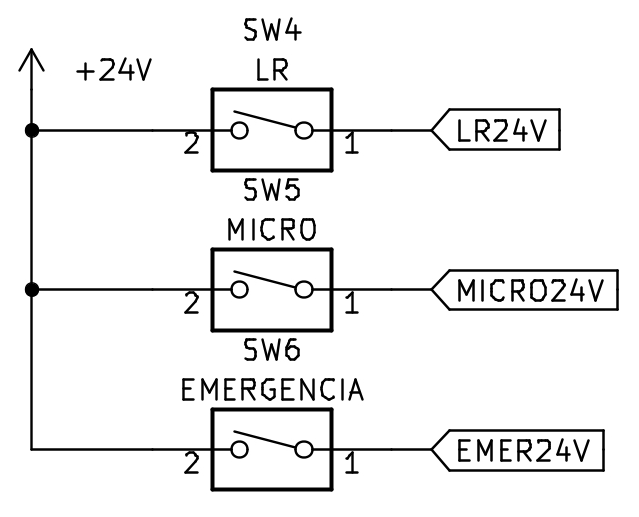
\includegraphics[scale=1.25]{03-placa/switches.png}
    \caption{Switches de estado}
    \label{fig:figura32switches}
    \end{figure}

Además, se cuenta con dos entradas digitales que deben ser capaces de mover el motor en el caso de que el
sistema se encuentre funcionando sin microcontrolador. Para ello estas señales deben actuar sobre los
pines de dirección del L298N. Estas dos señales son:
\begin{itemize}
    \item Avance (AVANCE). Actúa sobre el pin IN1 o IN3 del L298N.
    \item Retroceso (RETR). Actúa sobre el pin IN2 o IN4 del L298N.
\end{itemize}

Las señales se generan a 24V por defecto, por lo que es necesario su paso a 5V. Para ello se utilizan
optoacopladores, unos dispositivos que mediante fotodiodos acoplados a fototransistores. En este proyecto
se utiliza el circuito integrado TLP621-4 que cumple dicha función.

\begin{figure}[hbtp]
    \centering
    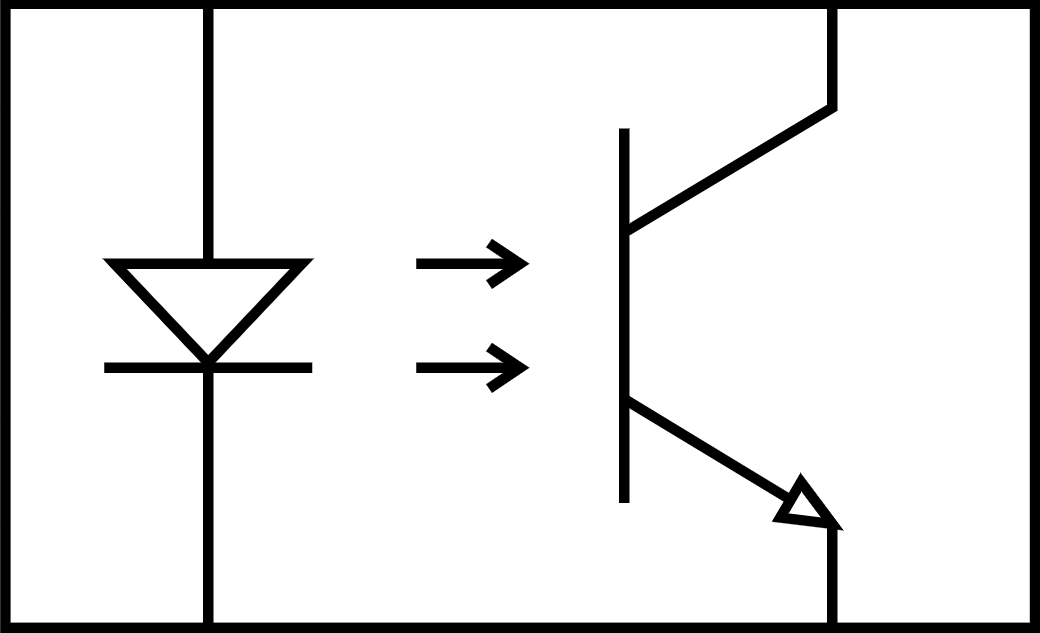
\includegraphics[width=\textwidth/4]{03-placa/02-optoac.png}
    \caption{Ejemplo de optoacoplador}
    \label{fig:figura33ejopto}
    \end{figure}

\subsection{Conversión de 24V a 5V}

En la figura \ref{fig:figura34imp} se muestra el circuito empleado. Se utiliza un total de dos TLP621-4 para
tener un total de 8 optoacopladores. Como la tensión máxima que reciben los diodos es de 24V, se colocan
unas resistencias para evitar que se quemen. El valor de las resistencias utilizadas es de 8.2 k$\Omega$,
permitiendo que la corriente directa sea algo inferior a 3 mA. Como caso relevante, en el caso de la parada
de emergencia, la resistencia será de 4.7 k$\Omega$ para que tenga una corriente directa y, una mayor
salida por ello para asegurar que se produzca la parada en caso de ser necesaria.

\begin{figure}[hbtp]
    \centering
    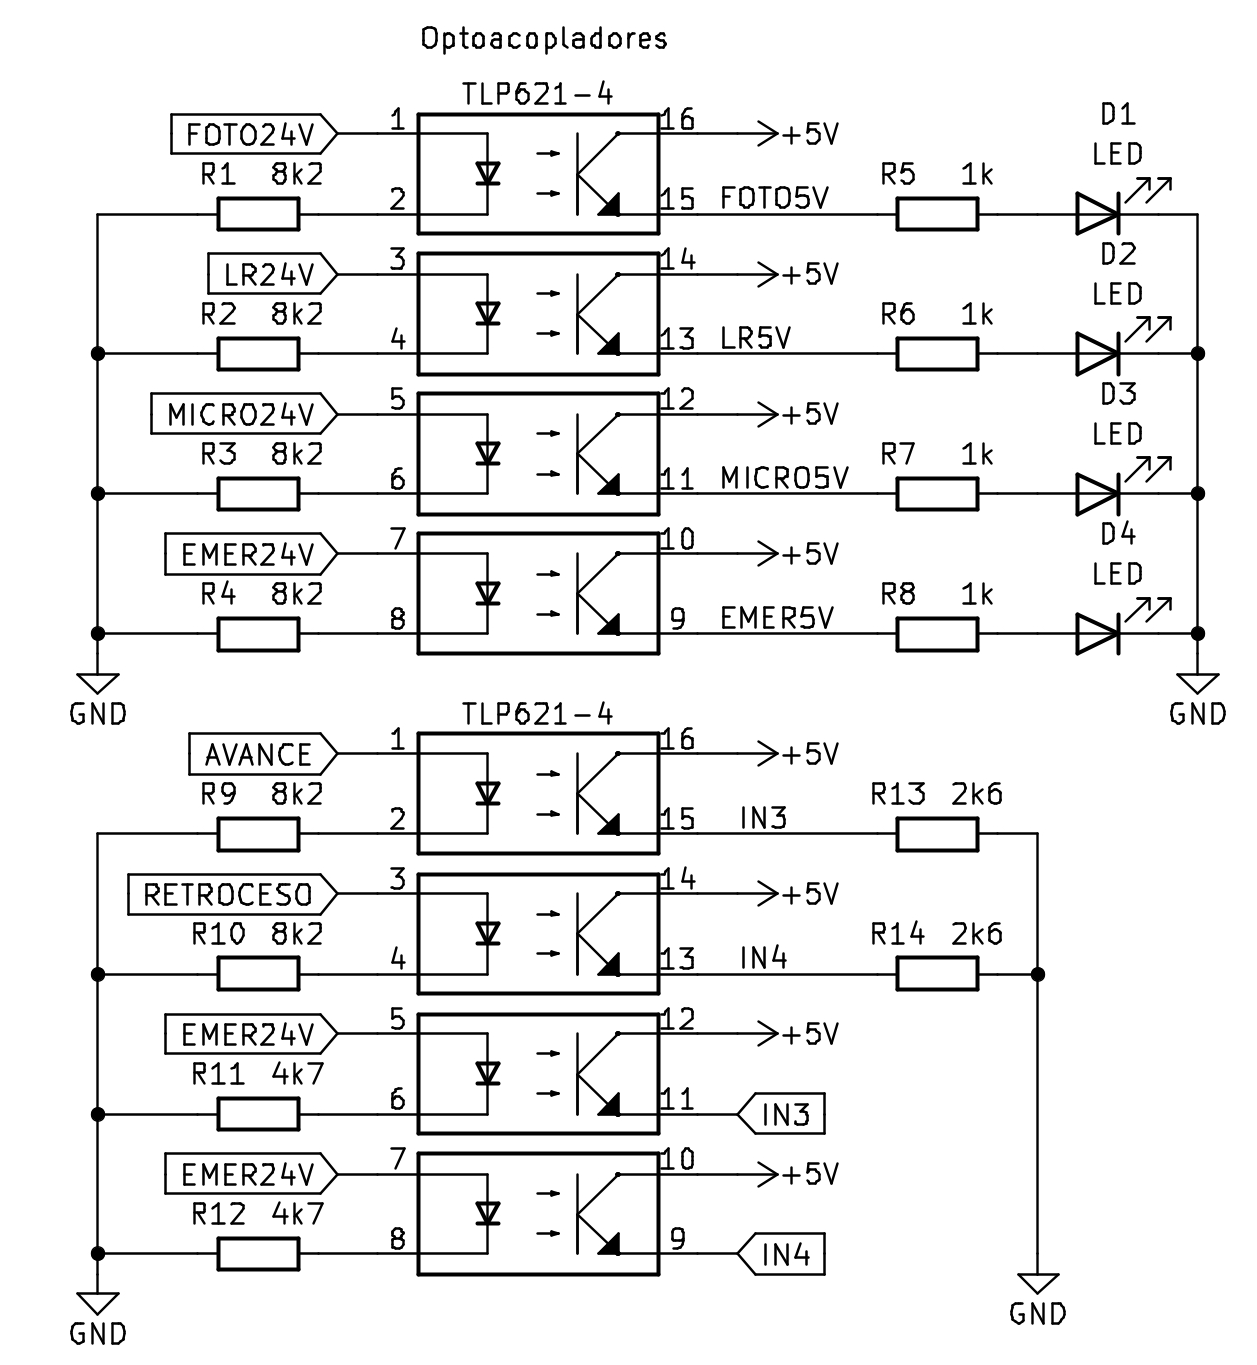
\includegraphics[scale=1.25]{03-placa/03-optoacopladores.png}
    \caption{Implementación de optoacopladores}
    \label{fig:figura34imp}
    \end{figure}

En el colector de los fototransistores se conectan directamente la línea de 5V para que, en caso de que la
señal correspondiente se active, su equivalente de 5V también lo haga. En las señales FOTO, LR, MICRO y EMER
se les añade un LED a la salida a modo de test para comprobar su funcionalidad, pero no se verán desde fuera
de la caja.

\subsection{Función sin microcontrolador y emergencia}

El sistema debe funcionar tanto con como sin el microcontrolador, por lo que la parte en la que no funcione
debe tener conexiones simples hacia la placa L298N. Para ello, cuando la señal MICRO sea un '1', se debe 
actuar sobre este dispositivo. Para evitar conflictos cuando el Arduino se encuentre conectado en este modo,
los pines conectados a IN3, IN4 y ENB se configurarán como entrada, ya que como salida generarán conflictos.

En primer lugar, se actúa sobre el pin controlador de la velocidad de giro, ENB (o ENA). Para ello, mediante
un búfer de tensión, se activa dicha señal al máximo cuando MICRO se encuentre en '1'. El búfer de tensión
se utiliza para independizar la salida a ENB de la señal MICRO de 5V y permitir su uso con el Arduino en otros modos.
La implementación se muestra en la figura \ref{fig:buferenb}. Para dicho búfer de tensión se emplea un canal
del circuito integrado TL082.

\begin{figure}[hbtp]
    \centering
    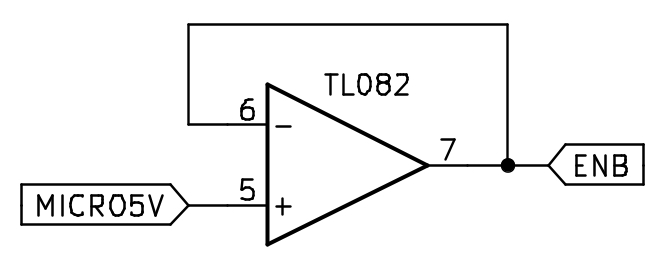
\includegraphics[scale=1.25]{03-placa/buferenb.jpg}
    \caption{Búfer de tensión de la señal MICRO a 5V}
    \label{fig:buferenb}
    \end{figure}

Para dar señal de movimiento se utilizan las flechas presentes en la caja. Estas flechas de selección tienen
dos salidas independientes, por lo que las señales lógicas que recibe el Arduino pueden ir por un canal 
mientras que la señal de movimiento en modo sin microcontrolador por otro. De este modo, si las señales de 
movimiento se utilizan a 24V se puede conectar directamente al panel de señales digitales remoto, el cual
interactúa directamente con la controladora del robot. Por ello, el terminal común que conecta la flecha de 
selección para el modo sin microcontrolador va conectado a la señal MICRO de 24V como se ve en la figura
\ref{fig:flecha}.

\begin{figure}[hbtp]
    \centering
    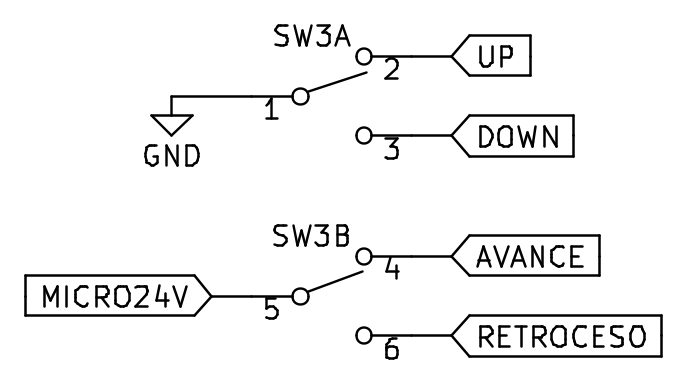
\includegraphics[scale=1.25]{03-placa/flecha.jpg}
    \caption{Conexiones flecha selección}
    \label{fig:flecha}
    \end{figure}

Por último, para que se produzca el movimiento además se debe actuar sobre IN3 o IN4 para que el motor se
mueva hacia un lado o hacia el otro. Para ello, se vuelven a utilizar optoacopladores como se ve en la
figura \ref{fig:sinmicro}. La señal de AVANCE y la señal de RETROCESO actúa sobre el optoacoplador que
le corresponde y pone el pin que le corresponde a '1', haciendo que el motor se mueva en el sentido deseado.
Como la flecha solo activa uno de los dos sentidos cada vez, no se producirá el bloqueo del motor.

Sin embargo, interesa que se produzca dicho bloqueo en un determinado caso: la parada de emergencia. Si tanto
IN3 como IN4 se ponen a '1' a la vez, el motor queda totalmente bloqueado y deja de moverse. Por ello, para
ello, se conecta la señal EMER de 24V a dos optoacopladores independientes que, en caso de que sea necesario,
produzca dicha parada. La misma se realizará tanto en modo sin microcontrolador como con éste activo, ya que 
depende directamente de la señal EMER.

\begin{figure}[hbtp]
    \centering
    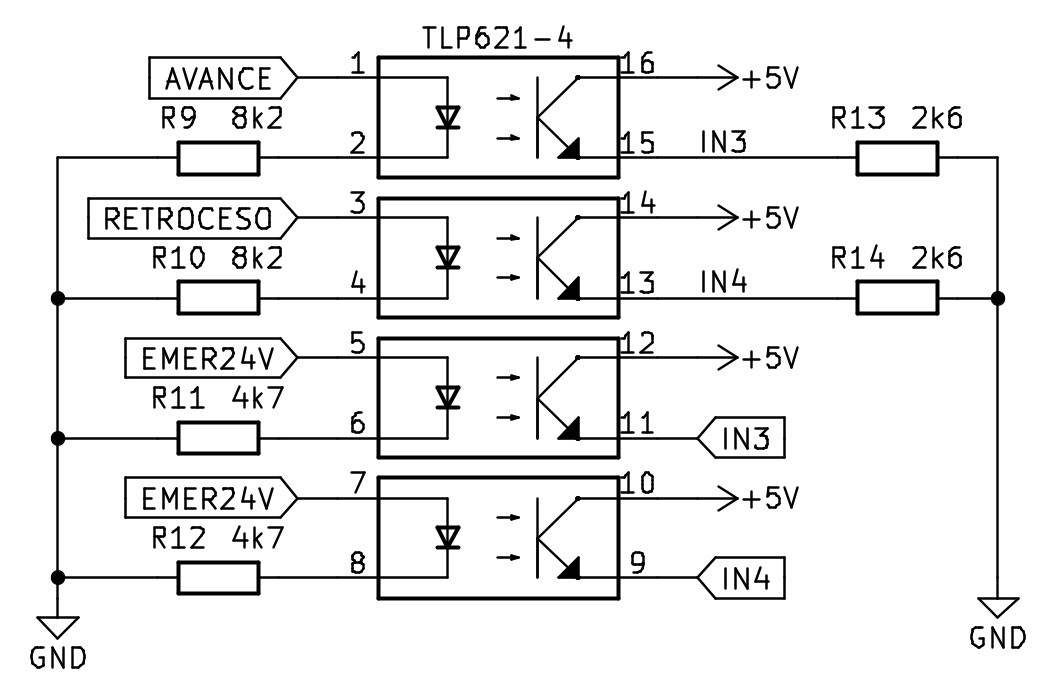
\includegraphics[scale=1.25]{03-placa/sinmicro.jpg}
    \caption{Implementación de optoacopladores para modo sin microcontrolador y emergencia}
    \label{fig:sinmicro}
    \end{figure}

\section{Calibre digital}

\subsection{Alimentación calibre}

Para el funcionamiento del calibre digital, éste debe ser alimentado por una fuente de 1.5V. Como lo que se
dispone en este proyecto es de 5V y 24V lo más sencillo es colocar un divisor resistivo a la línea de 5V y
utilizar un búfer de tensión para mantener dicho nivel lógico estable. Utilizando resistencias lo suficientemente
altas el consumo es despreciable. Por ello se utiliza una resistencia de 39k$\Omega$ y otra de 100k$\Omega$. La 
tensión de salida obtenida será de:

\begin{equation}
    V_{out} = 5V \frac{39k\Omega}{39k\Omega+100k\Omega} \approx 1.4V
\end{equation}

Los 1.4V que se obtienen entran dentro del rango de funcionamiento del calibre utilizando resistencias comerciales,
por lo que el resultado es válido. 

El consumo del divisor resistivo por otro lado será de:

\begin{equation}
    I_{divisor} = \frac{5V}{39k\Omega+100k\Omega} \approx 0.036 mA
\end{equation}

Se puede considerar un consumo despreciable.

\begin{figure}[hbtp]
    \centering
    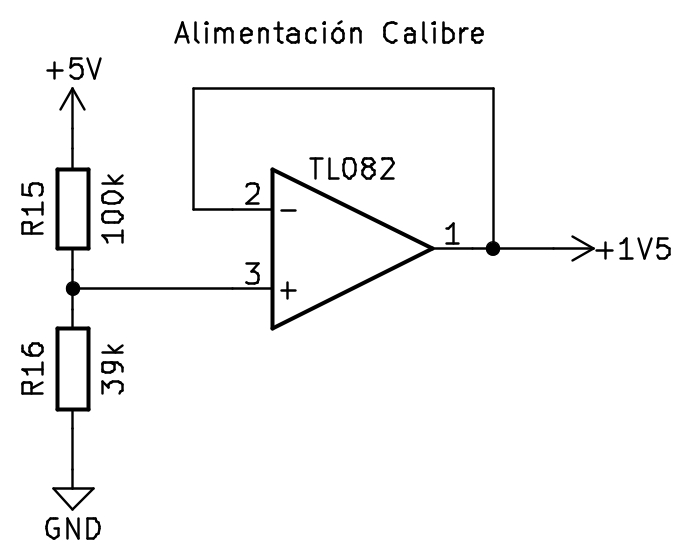
\includegraphics[width=\textwidth/2]{03-placa/04-alimentacion-calibre.png}
    \caption{Alimentación calibre digital a 1.5V}
    \label{fig:alimcal}
\end{figure}

Para el búfer de tensión se utiliza un circuito integrado TL082, del cual se utiliza uno de los dos amplificadores
operacionales con el que cuenta. Como resultado se obtiene el circuito de la figura \ref{fig:alimcal}.

\subsection{Amplificación señales calibre}

Para la lectura de la señal del calibre por parte del Arduino es necesario elevar los niveles de tensión a 5V.
Para ello se toma como referencia el circuito visto en la web \cite{caliper}. Éste utiliza un transistor junto
con dos resistencias de modo que cuando el calibre envíe un '1' se eleve la tensión a 5V, pero sin distorsionarse
cuando haya un '0' y dar falsos positivos. El esquema implementado es el que aparece en la figura \ref{fig:figura36amp}.

\begin{figure}[hbtp]
    \centering
    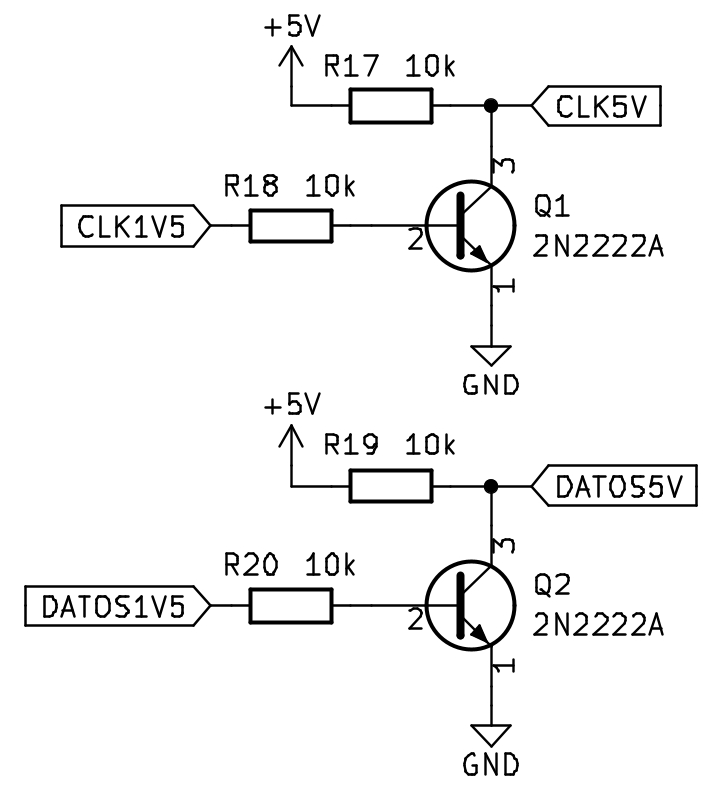
\includegraphics[width=\textwidth/2]{03-placa/05-amplificacion-calibre.png}
    \caption{Amplificación señales calibre digital a 5V}
    \label{fig:figura36amp}
    \end{figure}

\section{Placas finales}

Una vez descrita la funcionalidad del sistema electrónico a implementar, el resto del proceso consiste en 
separar las conexiones entre las placas de circuito impreso y determinar qué va conectado a cada una.

\subsection{Placa \textit{Tapa}}

La placa \textit{Tapa} como su propio nombre indica irá colocada en la superficie superior de la caja. Su 
principal función es permitir que la caja se pueda abrir sin que haya peligro de desconexiones ni tirones
entre los cables que conectan los distintos dispositivos que se encuentren en la tapa. Para ello, habrá
ristra de cables que se conecte a al fondo de la caja directamente y así simplificarlo todo.

Por otro lado, los dispositivos que van conectados a esta tapa son los destinados a ser la interfaz 
hombre-máquina. Estos dispositivos son:
\begin{itemize}
    \item LCD.
    \item Seta de emergencia.
    \item Botón intro y escape.
    \item Flecha de selección.
    \item Interruptores de estado (LR y MICRO)
\end{itemize}

El resultado final se puede observar en la figura \ref{fig:placatapa}. En ésta se puede observar los 
huecos para soldar los futuros conectores atornillables. Cuenta con dos zonas diferenciadas como se 
comentó previamente: una para la conexión de los dispositivos y otra para la conexión a la placa del 
fondo.

\begin{figure}[htpb]% 
    \centering 
    \subfloat[][]{% 
        \label{fig:tapafrente}% 
        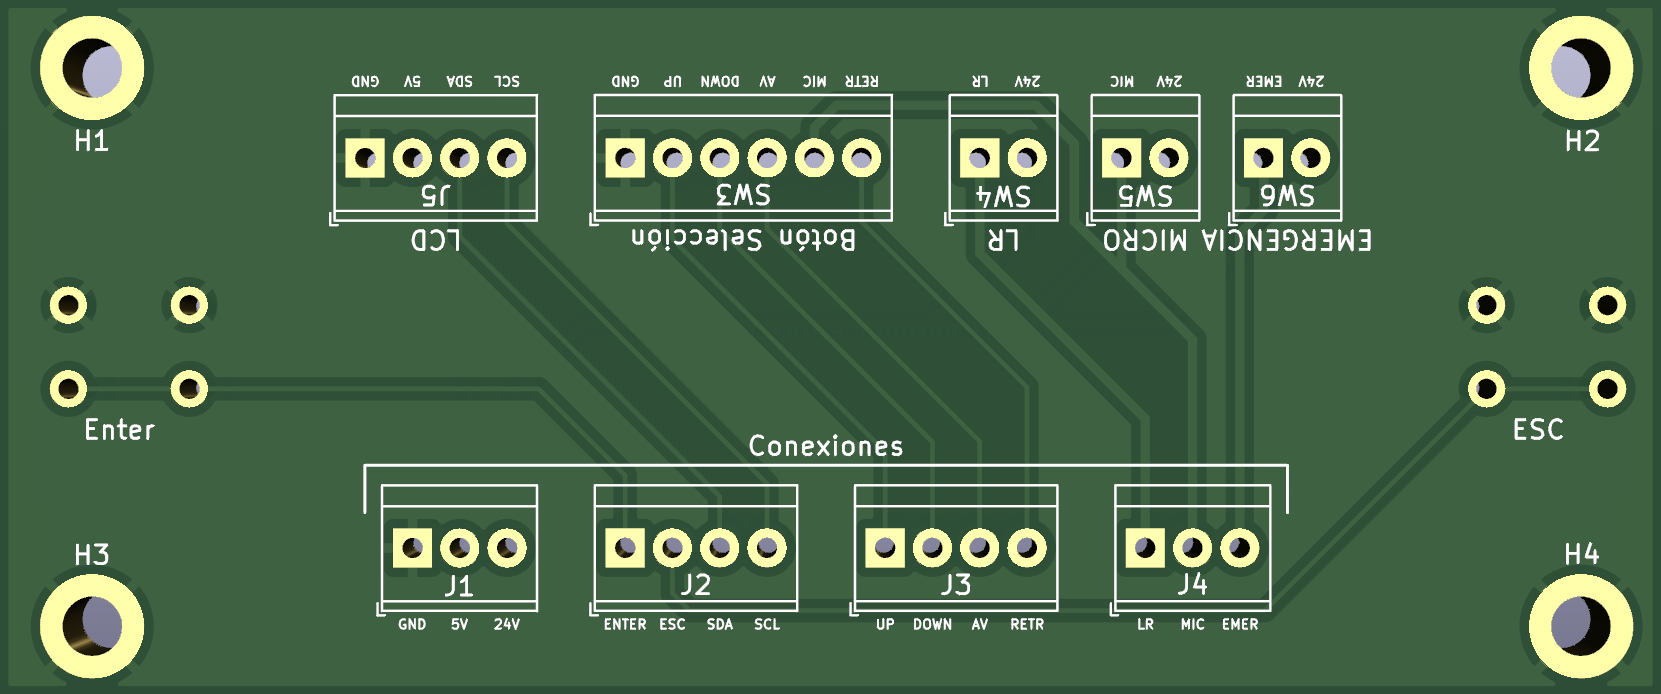
\includegraphics[scale=0.15]{03-placa/tapafrente.png}
    }% 
    \hspace{10pt}% 
    \subfloat[][]{% 
        \label{fig:tapatras}% 
        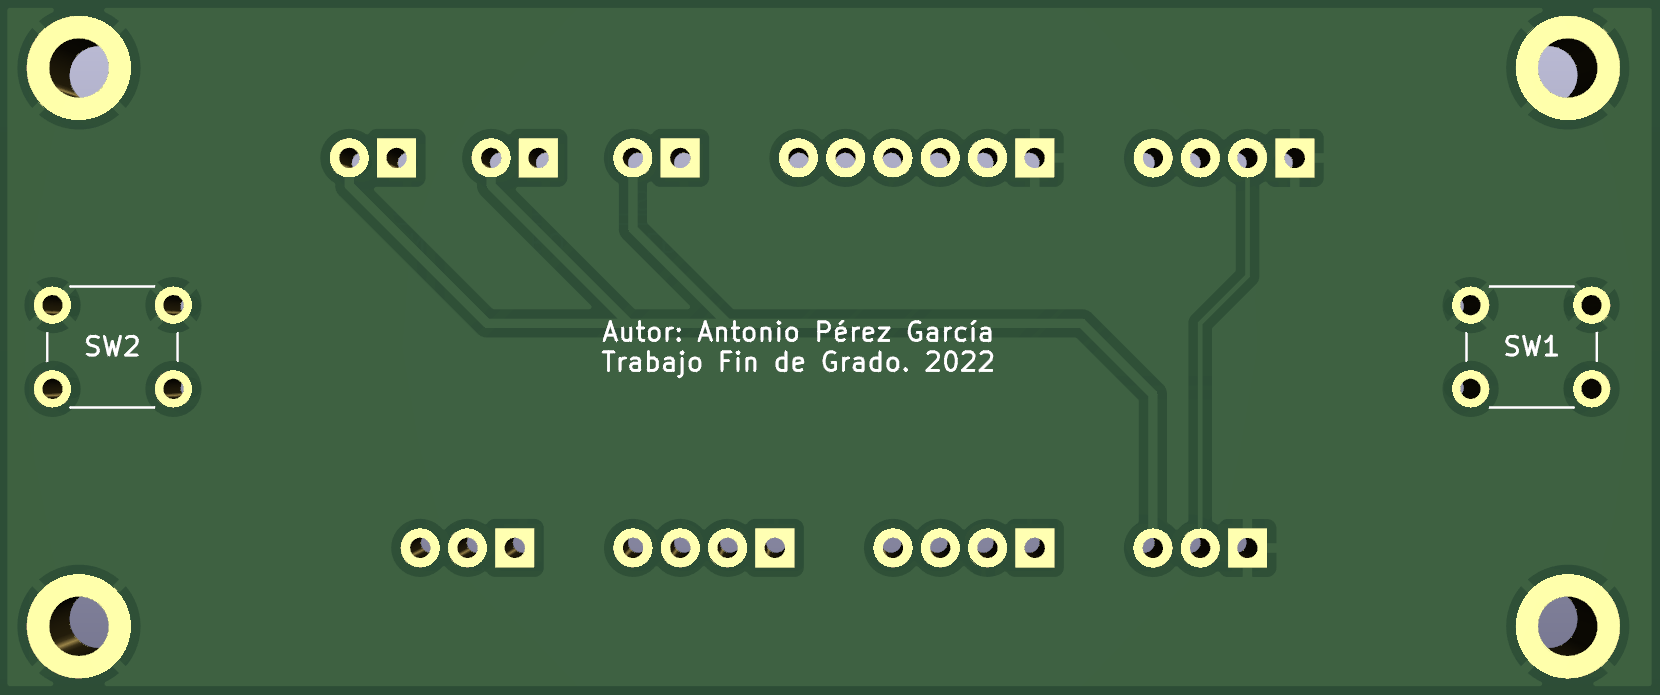
\includegraphics[scale=0.15]{03-placa/tapatras.png}
    }
    \caption{a) Vista frontal de la placa tapa. b) Vista trasera de la placa tapa}
    \label{fig:placatapa} 
    \end{figure} 

Como se puede observar, originalmente hay hueco para que los botones sean soldados en la propia placa ya 
que estaba pensado otra distribución, pero que posteriormente fueron sustituidos, por lo que en dichos 
huecos se sustituye por conectores atornillables.
    
\subsection{Placa \textit{Fondo}}

La placa \textit{Fondo} va situada en la base de la caja junto con el resto de dispositivos. Ésta se encarga
de realizar las funciones indicadas en los puntos anteriores de este capítulo, además de ser el centro neurálgico
del proyecto donde se producen todas las conexiones. En la figura \ref{fig:placafondo} se ve el resultado final.

\begin{figure}[htpb]% 
    \centering 
    \subfloat[][]{% 
        \label{fig:fondofrente}% 
        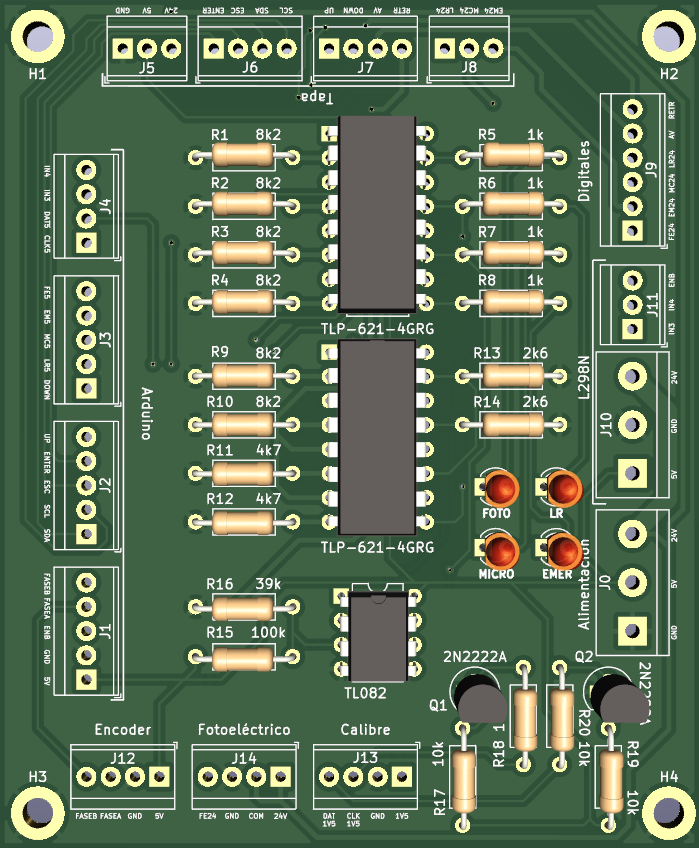
\includegraphics[scale=0.29]{03-placa/fondofrente.png}
    }% 
    \hspace{10pt}% 
    \subfloat[][]{% 
        \label{fig:fondotras}% 
        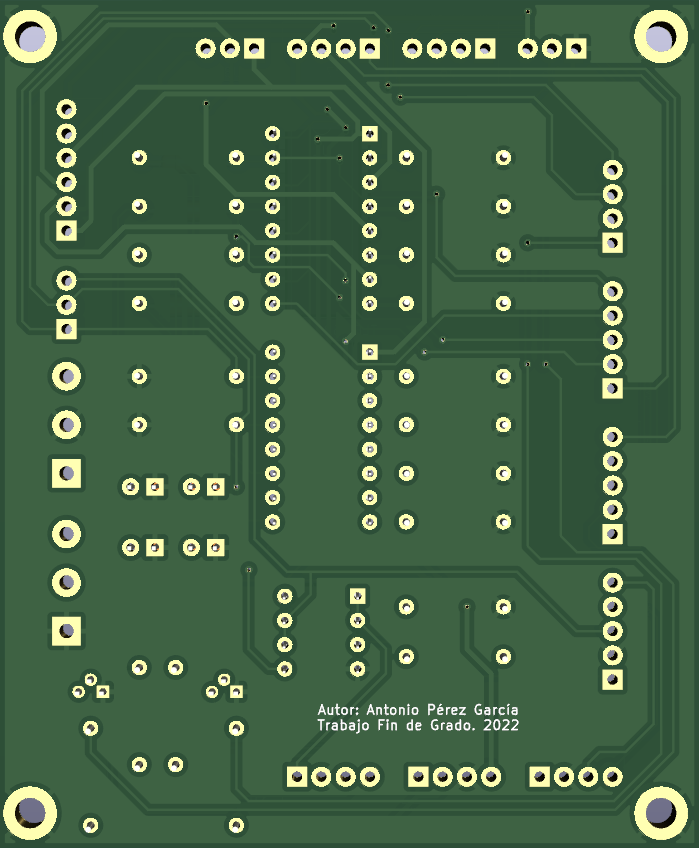
\includegraphics[scale=0.29]{03-placa/fondotras.png}
    }
    \caption{a) Vista frontal de la placa fondo. b) Vista trasera de la placa fondo}
    \label{fig:placafondo} 
    \end{figure} 

En la figura se puede diferenciar varias zonas:

\begin{itemize}
    \item Conexiones a la tapa en la zona superior.
    \item Conexiones al Arduino en la zona izquierda.
    \item Alimentación, conexiones a L298N y pines digitales en la zona derecha.
    \item Conexiones a los dispositivos (encoder, calibre y sensor fotoeléctrico) en la zona inferior.
    \item Zona central. Dedicada a realizar todas las interconexiones y las funciones que se han 
    indicado durante el capítulo.
\end{itemize}